\documentclass{beamer}
%\usetheme{Boadilla}
\usetheme{DarkConsole}
\usepackage[backend=biber]{biblatex}
\addbibresource{ref.bib}
\usepackage{courier}
\usepackage[T1]{fontenc}
\usepackage{multicol}
\usepackage{ifthen}
\usepackage{tikz}
\usepackage{hyperref}
\usetikzlibrary{calc}
\usepackage{graphicx}
\usepackage{listings}

\definecolor{myblack}{RGB}{68,68,68}
\definecolor{mygreen}{RGB}{64,128,0}
\setbeamercolor{block title}{bg=mygreen,fg=white}
\setbeamercolor{block body}{bg=myblack,fg=white}
%\addtobeamertemplate{block begin}{%
%  \setlength{\textwidth}{0.9\textwidth}%
%}{}
%\setbeamertemplate{blocks}[rounded][shadow]

\newcommand{\makens}[2]{
	\coordinate (#1) at (1.5,0);
	\coordinate (N#1) at ($(#1) + (0,1.8)$);
	\node at (N#1) {#1};
	\node (rect) at (#1) [draw,thick,minimum width=3.5cm,minimum height=3cm] {};
	\coordinate (#2) at ($(N#1) + (0,2)$);
	\coordinate (N#2) at ($(#2) + (0,1.8)$);
	\node at (N#2) {#2};
	\node (rect) at (#2) [draw,thick,minimum width=3.5cm,minimum height=3cm] {};
}

\newcommand{\makenode}[5]{
	\coordinate (#3) at (#4,#5);
	\coordinate (T#3) at ($(#3) + (0,1.3)$);
	\coordinate (B#3) at ($(#3) - (0,1.3)$);
	\node at (#3) [draw,thick,minimum width=2cm,minimum height=2cm] {};
	\node at (T#3) {#1};
	\ifthenelse { \equal {#2} {} }
	{}
	{
		\node at (#3) {
			\includegraphics[width=0.1\textwidth]{#2}
		};
	}
}

\newcommand{\makevnode}[5]{
	\coordinate (#3) at (#4,#5);
	\coordinate (T#3) at ($(#3) + (0,3.3)$);
	\coordinate (B#3) at ($(#3) - (0,3.3)$);
	\node at (#3) [draw,thick,minimum width=2cm,minimum height=6cm] {};
	\node at (T#3) {#1};
	\ifthenelse { \equal {#2} {} }
	{}
	{
		\node at (#3) {
			\includegraphics[width=0.1\textwidth]{#2}
		};
	}
}


\graphicspath{ {./assets} }

\title {Kubernetes}
\author {Henrique Tsuyoshi Yara}
\institute {OPUS-software}

\begin{document}

\begin{frame}{\titlepage}
	\begin{figure}[htpb]
		\centering
		
\includegraphics[width=0.5\textwidth]{Kubernetes_logo}
		\caption{Kubernetes logo}
	\end{figure}
\end{frame}

\begin{frame}{Índice}
\begin{multicols}{2}
  \tableofcontents
\end{multicols}
\end{frame}

%\setbeamercovered{transparent}

\section{K8s}

\begin{frame}
\frametitle{Conceito}
\begin{itemize}
	\item O kubernetes provê:
		\begin{itemize}
			\item \uncover<2->{\textit{Service Discovery} e Balanceamento de carga}
			\item \uncover<3->{Orquestração de armazenamento}
			\item \uncover<4->{\textit{Rollouts} e \textit{Rollbacks} automáticos}
			\item \uncover<5->{Controle de recursos automáticos (CPU, RAM)}
			\item \uncover<6->{Auto recuperação}
			\item \uncover<7->{Gerenciamento de \textit{Secrets} e configurações}
		\end{itemize}
\end{itemize}

%Service discovery and load balancing Kubernetes can expose a container using the DNS name or using their own IP address. If traffic to a container is high, Kubernetes is able to load balance and distribute the network traffic so that the deployment is stable.
%Storage orchestration Kubernetes allows you to automatically mount a storage system of your choice, such as local storages, public cloud providers, and more.
%Automated rollouts and rollbacks You can describe the desired state for your deployed containers using Kubernetes, and it can change the actual state to the desired state at a controlled rate. For example, you can automate Kubernetes to create new containers for your deployment, remove existing containers and adopt all their resources to the new container.
%Automatic bin packing You provide Kubernetes with a cluster of nodes that it can use to run containerized tasks. You tell Kubernetes how much CPU and memory (RAM) each container needs. Kubernetes can fit containers onto your nodes to make the best use of your resources.
%Self-healing Kubernetes restarts containers that fail, replaces containers, kills containers that don't respond to your user-defined health check, and doesn't advertise them to clients until they are ready to serve.
%Secret and configuration management Kubernetes lets you store and manage sensitive information, such as passwords, OAuth tokens, and SSH keys. You can deploy and update secrets and application configuration without rebuilding your container images, and without exposing secrets in your stack configuration.

\end{frame}

\begin{frame}
\frametitle{Componentes}
\begin{itemize}
	\item \textit{Pod}: Consiste em um container ou um conjunto de containers
	\item \uncover<2->{\textit{Node}: É onde fica agrupado os \textit{Pods} que compõe a aplicação}
	\item \uncover<3->{\textit{Cluster}: Um conjunto de máquinas trabalhadoras (\textit{Nodes})}
	\item \uncover<4->{\textit{Control Plane}: Faz decisões e gerencia o \textit{cluster} (detectar eventos, programar \textit{pods})}
		\begin{itemize}
			\item \uncover<5->{Pode rodar em múltiplos nós provendo alta disponibilidade e prevenindo falhas}
		\end{itemize}
	\item \uncover<6->{\textit{Worker}: Máquinas trabalhadoras que vão rodar a aplicação(\textit{Nodes})}
		\begin{itemize}
			\item \uncover<7->{Geralmente são usados múltiplos nós \textit{workers} provendo alta disponibilidade e prevenindo falhas}
		\end{itemize}
\end{itemize}
\end{frame}

\begin{frame}
\frametitle{Componentes - \textit{Control Plane}}
\begin{itemize}
	\item \textbf{kube-apiserver}: \textit{front end} do \textit{control plane}. A implementação foi feita de uma forma que é possível ser escalada horizontalmente em várias instancias e consegue balancear o trafico de rede entre essas instâncias.
	\item \uncover<2->{\textbf{etcd}: Possui consistência e alta disponibilidade. Armazena os dados do cluster em valores-chaves. É bom ter um \textit{backup} para esses dados}
	\item \uncover<3->{\textbf{kube-scheduler}: Procura por \textit{Pods} que não foram atribuídos à nós e atribui nós para eles (Leva em conta políticas, \textit{hardware}, \textit{software}, etc\dots)}
\end{itemize}
\end{frame}

\begin{frame}
\frametitle{Componentes - \textit{Control Plane}}
\begin{itemize}
	\item \textbf{kube-controller-manager}: Roda processos \textit{controllers}
		\begin{itemize}
			\item \uncover<2->{\textbf{Node controller}: Verificar quando um nó falha}
			\item \uncover<3->{\textbf{Job controller}: Procuram por \textit{Job} que acontecem apenas uma vez, criam \textit{Pods} para executar a tarefa}
			\item \uncover<4->{\textbf{EndpointSlice controller}: Popula objetos \textit{EndpointSlice} (provê links entre Serviços e \textit{Pods})}
			\item \uncover<5->{\textbf{ServiceAccount controller}: Criar \textit{ServiceAccounts} para novos \textit{namespaces}}
		\end{itemize}
\end{itemize}
\end{frame}

\begin{frame}
\frametitle{Componentes - Todos os \textit{Nodes}}
Estão em todos os nós, fazem manutenção nos \textit{Pods} rodando.
\begin{itemize}
	\item \textbf{kubelet}: Garantem que os containers estão rodando em um \textit{Pod}
		\begin{itemize}
			\item \uncover<2->{O \textbf{kubelet} não gerencia containers que não foram criados pelo \textbf{kubernetes}}
		\end{itemize}
	\item \uncover<3->{\textbf{kube-proxy}: Um proxy que roda em todos os nós do \textit{cluster}}
		\begin{itemize}
			\item \uncover<4->{Fazem com que as regras de redes funcionem nos nós (Permitem comunicação de rede dos \textit{Pods} dentro e fora do cluster)}
		\end{itemize}
\end{itemize}
\end{frame}


\section{K8s vs Docker}

\begin{frame}
\frametitle{K8s vs Docker}
\begin{itemize}
	\item \textbf{Docker} é uma plataforma de containerização
	\item \textbf{K8s} é um orquestrador de containers
\end{itemize}
\end{frame}


\section{Pod vs Container}

\begin{frame}
\frametitle{Pods vs containers}
\textbf{"Pods are the smallest deployable units of computing that you can create and manage in Kubernetes."} \cite{K8s}
\begin{itemize}
	\item \uncover<2->{1 Pod : 1 Container}
	\item \uncover<3->{Grupo de 1 ou mais containers}
		\begin{itemize}
			\item \uncover<4->{Compartilham armazenamento e rede}
			\item \uncover<5->{Especificações para rodar o container}
			\item \uncover<6->{Pode conter initContainers}
			\item \uncover<7->{Pode conter containers efêmeros}
		\end{itemize}
\end{itemize}
\end{frame}

\begin{frame}
\frametitle{Containers efêmeros}
\textbf{Ephemeral containers}:
\begin{itemize}
	\item Geralmente é usado para inspecionar (\textit{Debugging}) o estado do Pod:
	\item \uncover<2->{Não possui portas, portanto \textbf{livenessProbe, readinessProbe} não são permitidos}
	\item \uncover<3->{Recursos do pod são imutáveis, portanto não é permitido configurar recursos}
	\item \uncover<4->{Lista completa de permissões: \href{https://kubernetes.io/docs/reference/generated/kubernetes-api/v1.26/\#ephemeralcontainer-v1-core}{link}}
\end{itemize}
\end{frame}

\begin{frame}
\frametitle{Pods estáticos}
\begin{itemize}
	\item Gerenciados diretamente pelo \textit{kubelet} do nó (indepentente do \textit{API server})
	\item \uncover<2->{O \textit{kubelet} verifica o \textit{Pod} e reinicia caso falhe}
	\item \uncover<3->{\textit{kubelet} verifica o diretório \textit{/etc/kubernetes/manifests} por padrão e cria pods caso seja necessário}
	\item \uncover<4->{Não suporta \textit{Containers efêmeros} e não pode referenciar outros objetos da \textit{API (ConfigMap, Secret, etc\dots)}}
	\item \uncover<5->{Onde usar?}
		\begin{itemize}
			\item \uncover<6->{Nos componentes do control plane\footnote{\url{https://anote.dev/static-pods-in-kubernetes/}}}
		\end{itemize}
\end{itemize}
\end{frame}

\begin{frame}
	\frametitle{\textit{LivenessProbe}, \textit{ReadinessProbe} e \textit{StartUpProbe}}

Os 3 são controlados pelo \textit{kubelet}

\uncover<2->{\textbf{LivenessProbe}:}
\begin{itemize}
	\item \uncover<2->{Tentar fazer a aplicação ficar mais disponível removendo \textit{bugs}}
		\begin{itemize}
			\item \uncover<3->{Pode perceber um \textit{deadlock} na aplicação}
		\end{itemize}
\end{itemize}
\end{frame}

\begin{frame}[containsverbatim]
\frametitle{\textit{LivenessProbe}, \textit{ReadinessProbe} e \textit{StartUpProbe}}
\begin{center}
\begin{minipage}{0.9\textwidth}
\begin{block}{Exemplo \textit{LivenessProbe}}
\begin{lstlisting}
livenessProbe:
  tcpSocket:
    port: 8080
  initialDelaySeconds: 60
  periodSeconds: 60
\end{lstlisting}
\end{block}
\end{minipage}
\end{center}
\end{frame}

\begin{frame}
	\frametitle{\textit{LivenessProbe}, \textit{ReadinessProbe} e \textit{StartUpProbe}}

\uncover<1->{\textbf{ReadinessProbe}:}
\begin{itemize}
	\item \uncover<1->{É usado para saber quando um container está pronto para aceitar tráfico de rede.}
	\begin{itemize}
		\item \uncover<2->{Pode ser usado para controlar os pods que servem como \textit{backend}}
		\item \uncover<3->{Se o pod não estiver pronto, ele é removido do \textit{Load Balancer} do serviço}
	\end{itemize}
\end{itemize}
\end{frame}

\begin{frame}[containsverbatim]
\frametitle{\textit{LivenessProbe}, \textit{ReadinessProbe} e \textit{StartUpProbe}}
\begin{center}
\begin{minipage}{0.9\textwidth}
\begin{block}{Exemplo \textit{ReadinessProbe}}
\begin{lstlisting}
readinessProbe:
  tcpSocket:
    port: 8080
  initialDelaySeconds: 60
  periodSeconds: 60
\end{lstlisting}
\end{block}
\end{minipage}
\end{center}
\end{frame}

\begin{frame}
\frametitle{\textit{LivenessProbe}, \textit{ReadinessProbe} e \textit{StartUpProbe}}
\textbf{StartupProbe}:
\begin{itemize}
	\item É usado para sabe se o container da aplicação começou.
	\begin{itemize}
		\item \uncover<2->{Pode ser configurado para desativar \textit{liveness} e \textit{readness} até o \textit{startup} tenha sucesso.}
		\item \uncover<3->{Dessa forma o \textit{kubelet} não vai matar aplicações lentas antes de elas inicializarem.}
	\end{itemize}
\end{itemize}
\end{frame}

\section{Cluster local}

\begin{frame}
\frametitle{Cluster Local}
\begin{itemize}
	\item \uncover<1->{Ambientes menores (Recursos da máquina local);}
	\item \uncover<2->{Para aprendizado;}
	\item \uncover<3->{Não são feitos para produção}
\end{itemize}
\end{frame}

\begin{frame}
\frametitle{Ferramentas}
Ferramentas para criação de cluster \textbf{local} do kubernetes:
\begin{itemize}
	\uncover<2->{\item kind (Kubernetes in Docker)
		\begin{itemize}
			\item Cluster usando containers de docker para criar os nós.
		\end{itemize}}
	\uncover<3->{\item kubeadm
		\begin{itemize}
			\item Cluster usando um container runtime.
		\end{itemize}}
	\uncover<4->{\item minikube
		\begin{itemize}
			\item Cluster usando containeres ou máquinas virtuais.
		\end{itemize}}
\end{itemize}
\end{frame}

\begin{frame}[containsverbatim]
\frametitle{Criando o cluster com minikube}
Criação do cluster utilizado na parte prática:
\begin{center}
\begin{minipage}{0.9\textwidth}
\begin{block}{Comando \textit{minikube}}
\begin{lstlisting}[language=bash]
minikube start --nodes='4' \
--network-plugin=cni \
--cni=calico \
--profile=multinode \
--vm-driver=virtualbox \
--kubernetes-version=v1.24.3
\end{lstlisting}
\end{block}
\end{minipage}
\end{center}
\end{frame}

\begin{frame}
\frametitle{Nós}
\centering
\begin{multicols}{2}
	\begin{tikzpicture}
		\node at (-0.5,0) {};
		\node (PC1) at (3.6,2) [draw,thick,minimum width=8cm,minimum height=7.5cm] {};
		\node at ($(PC1) + (0,4.05)$) {Computador 1};
		\makenode{Master}{}{M}{1}{3.5}
		\node at ($(M) + (0,0)$) {\huge K8s};
		\node at (BM) {\tiny 192.168.59.154};
		\makenode{Qualquer nó}{}{Q}{1}{0}
		\node at ($(Q) + (0,0.5)$) {\tiny Ingress-};
		\node at ($(Q) + (0,0)$) {\tiny controller};
		\node at ($(Q) + (0,-0.5)$) {\tiny Ingress-dns};
		\coordinate (W2) at (5,3.5);
		\coordinate (TW2) at ($(W2) + (0,1.3)$);
		\coordinate (BW2) at ($(W2) - (0,1.3)$);
		\node at (W2) [draw,thick,minimum width=4.5cm,minimum height=2cm] {};
		\node at (TW2) {M02};
		\node at ($(W2) + (1,0)$) {
\includegraphics[width=0.1\textwidth]{MariaDB}};
		\node at ($(W2) - (1,0)$) {
\includegraphics[width=0.1\textwidth]{Redis}};
		\makenode{M03}{}{W3}{6.25}{0}
		\node at ($(W3) + (0.4,0)$) {
\includegraphics[width=0.05\textwidth]{Apache}};
		\node at ($(W3) - (0.4,0)$) {
\includegraphics[width=0.05\textwidth]{CTFd}};
		\makenode{M04}{Php}{W4}{3.75}{0}
		\node at (BW2) {\tiny 192.168.59.155};
		\node at (BW3) {\tiny 192.168.59.156};
		\node at (BW4) {\tiny 192.168.59.157};
	\end{tikzpicture}
	\columnbreak
	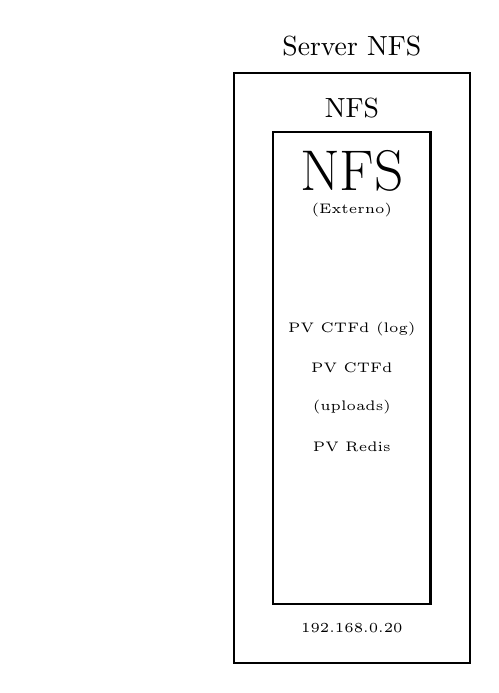
\begin{tikzpicture}
		\node at (-4,0) {};
		\node (PC1) at (0,0) [draw,thick,minimum width=3cm,minimum height=7.5cm] {};
		\node at ($(PC1) + (0,4.085)$) {Server NFS};
		\makevnode{NFS}{}{NFS}{0}{0}
		\node at (BNFS) {\tiny 192.168.0.20};
		\node at ($(NFS) + (0,2.5)$) {\huge NFS};
		\node at ($(NFS) + (0,2)$) {\tiny (Externo)};
		\node at ($(NFS) + (0,0.5)$) {\tiny PV CTFd (log)};
		\node at ($(NFS) + (0,0)$) {\tiny PV CTFd};
		\node at ($(NFS) + (0,-0.5)$) {\tiny (uploads)};
		\node at ($(NFS) + (0,-1)$) {\tiny PV Redis};
	\end{tikzpicture}
\end{multicols}
\end{frame}

\section{Recursos}

\begin{frame}
\frametitle{Recursos - Namespaces}

\begin{itemize}
	\item Os \textit{namespaces} permitem isolar grupos de recursos em um cluster
		\begin{itemize}
			\item \uncover<2->{Os \textit{namespaces} são uma forma de dividir o cluster para várias pessoas com limite de recursos.\footnote{\href{https://kubernetes.io/docs/concepts/overview/working-with-objects/namespaces/}{Kubernetes Documentation}}}
			\item \uncover<3->{Os administradores do cluster devem dividir os recursos}
		\end{itemize}
	\item \uncover<4->{O nome dos recursos precisam ser únicos em cada namespace}
	\item \uncover<5->{Não são todos os objetos que aceitam o isolamento do \textit{namespace}}
\end{itemize}
\end{frame}

\begin{frame}[containsverbatim]
\frametitle{Recursos - Namespaces}

Para ver os recursos que são e não são isolados por namespace

\begin{center}
\begin{minipage}{0.9\textwidth}
\begin{block}{\textbf{values.yaml}}
\begin{lstlisting}[language=bash]
# In a namespace
kubectl api-resources --namespaced=true

# Not in a namespace
kubectl api-resources --namespaced=false
\end{lstlisting}
\end{block}
\end{minipage}
\end{center}
\end{frame}

\begin{frame}
\frametitle{Namespaces}
\centering
\begin{multicols}{3}
	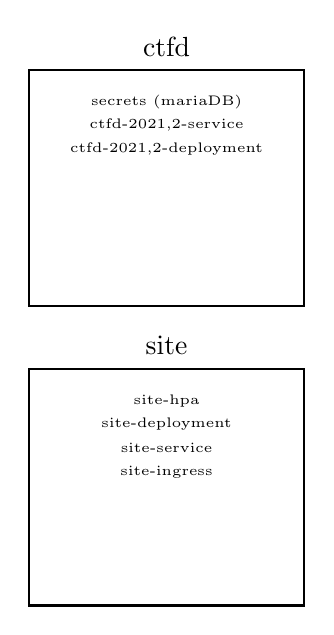
\begin{tikzpicture}
		\makens{site}{ctfd}
		\node (L1) at ($(site) + (0,1.1)$) {\tiny site-hpa};
		\node (L2) at ($(L1) - (0,0.3)$) {\tiny site-deployment};
		\node (L3) at ($(L2) - (0,0.3)$) {\tiny site-service};
		\node (L4) at ($(L3) - (0,0.3)$) {\tiny site-ingress};
		\node (L1) at ($(ctfd) + (0,1.1)$) {\tiny secrets (mariaDB)};
		\node (L2) at ($(L1)  - (0,0.3)$) {\tiny ctfd-202{1,2}-service};
		\node (L3) at ($(L2)  - (0,0.3)$) {\tiny ctfd-202{1,2}-deployment};
	\end{tikzpicture}
	\columnbreak
	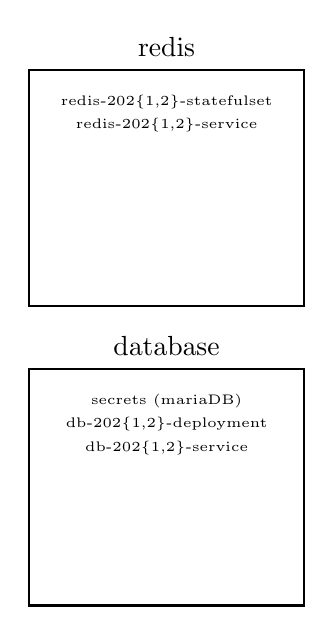
\begin{tikzpicture}
		\makens{database}{redis}
		\node (L1) at ($(database) + (0,1.1)$) {\tiny secrets (mariaDB)};
		\node (L2) at ($(L1) - (0,0.3)$) {\tiny db-202\{1,2\}-deployment};
		\node (L3) at ($(L2) - (0,0.3)$) {\tiny db-202\{1,2\}-service};
		\node (L1) at ($(redis) + (0,1.1)$) {\tiny redis-202\{1,2\}-statefulset};
		\node (L2) at ($(L1) - (0,0.3)$) {\tiny redis-202\{1,2\}-service};
	\end{tikzpicture}
	\columnbreak
	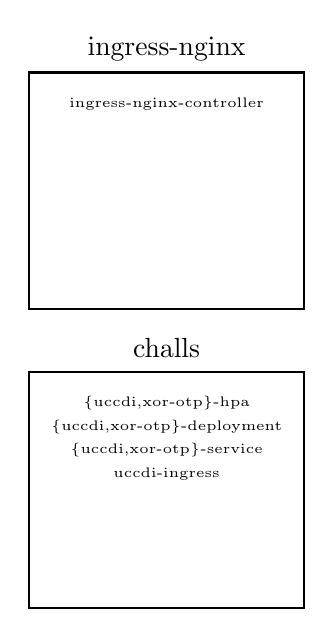
\begin{tikzpicture}
	\makens{challs}{ingress-nginx}
		\node (L1) at ($(challs) + (0,1.1)$) {\tiny \{uccdi,xor-otp\}-hpa};
		\node (L2) at ($(L1) - (0,0.3)$) {\tiny \{uccdi,xor-otp\}-deployment};
		\node (L3) at ($(L2) - (0,0.3)$) {\tiny \{uccdi,xor-otp\}-service};
		\node (L4) at ($(L3) - (0,0.3)$) {\tiny uccdi-ingress};
		\node (L1) at ($(ingress-nginx) + (0,1.1)$) {\tiny ingress-nginx-controller};
	\end{tikzpicture}
\end{multicols}
\end{frame}

\begin{frame}
\frametitle{Recursos - Daemonsets}
\begin{itemize}
	\item O \textit{DaemonSet} garante que todos os nós ou os nós selecionados rodem uma cópia de um \textit{Pod}
	\item \uncover<2->{Quando nós são adicionados nos clusters, os \textit{Pods} são adicionados nesses nós e vice versa}
	\item \uncover<3->{Deletar o \textit{DaemonSet} mata os \textit{Pods} que foram criados}
	\item \uncover<4->{Alguns exemplos de uso:}
	\begin{itemize}
		\item \uncover<4->{Rodar um \textit{cluster storage daemon} em todos os nós}
		\item \uncover<5->{Rodar um \textit{logs collection daemon} em todos os nós}
		\item \uncover<6->{Rodar um \textit{node monitoring daemon} em todos os nós}
	\end{itemize}
\end{itemize}
\end{frame}

\begin{frame}
\frametitle{Recursos - ConfigMaps}
\begin{itemize}
	\item O \textit{ConfigMap} é usado para guardar dados não confidenciais em pares de chave-valor
	\item \uncover<2->{Pode ser usado como:}
		\begin{itemize}
			\item \uncover<3->{Variáveis de ambiente}
			\item \uncover<4->{Argumentos de comando de linha}
			\item \uncover<5->{Arquivos de configuração em um volume}
		\end{itemize}
\end{itemize}
\end{frame}

\begin{frame}[containsverbatim]
\frametitle{Recursos - ConfigMaps}
\begin{itemize}
	\item Aplicação no projeto prático:
\begin{center}
\begin{minipage}{0.9\textwidth}
\begin{block}{Variáveis de ambiente}
\begin{lstlisting}
apiVersion: v1
kind: ConfigMap
metadata:
  name: ctfd-env-configmap
  namespace: ctfd
data:
  DB_FILE: '/etc/ctfd-db/database'
  DB_USER_FILE: '/etc/ctfd-db/username'
  DB_PASS_FILE: '/etc/ctfd-db/password'
  ACCESS_LOG: '-'
  ERROR_LOG: '-'
  UPLOAD_FOLDER: '/var/uploads'
  LOG_FOLDER: '/var/log/CTFd'
  REVERSE_PROXY: 'true'
\end{lstlisting}
\end{block}
\end{minipage}
\end{center}
\end{itemize}
\end{frame}

\begin{frame}
\frametitle{Recursos - Secrets}

\begin{itemize}
	\item O \textit{secret} é um objeto que contém uma pequena quantidade de dados \textbf{sensíveis}
	\item \uncover<2->{Como senhas, tokens, chaves, etc\dots}
	\item \uncover<3->{Dessa forma não é preciso incluir dados confidenciais no seu código}
	\item \uncover<4->{Algumas boas práticas para manter o \textit{secrets} seguro:\footnote{\url{https://kubernetes.io/docs/concepts/security/secrets-good-practices/}}}
		\begin{itemize}
			\item \uncover<4->{Encryption at Rest for Secrets}
			\item \uncover<5->{Enable or configure RBAC rules with least-privilege access to Secrets}
			\item \uncover<6->{Restrict Secret access to specific containers}
			\item \uncover<7->{Consider using external Secret store providers}
		\end{itemize}
\end{itemize}
\end{frame}

\begin{frame}[containsverbatim]
\frametitle{Recursos - Secrets}
\begin{itemize}
	\item Aplicação no projeto prático:
\begin{center}
\begin{minipage}{0.9\textwidth}
\begin{block}{Volumes}
\begin{lstlisting}
apiVersion: v1
kind: Secret
metadata:
  name: ctfd-db-2022
  namespace: database
type: Opaque
data:
  database: 'Y3RmZGRiCg=='
  username: 'Y3RmZHVzZXIK'
  password: 'Y3RmZHBhc3MK'
  root-pass: 'Y3RmZHJvb3RwYXNzCg=='
\end{lstlisting}
\end{block}
\end{minipage}
\end{center}
\end{itemize}
\end{frame}

\begin{frame}
\frametitle{Recursos - Services}
\begin{itemize}
	\item Os \textbf{Services} conseguem abstrair a parte da rede dos \textbf{Pods}
	\item \uncover<2->{Os \textbf{Services} cuidam da parte do balanceamento de carga e \textbf{Service Discovery}}
\end{itemize}
\end{frame}

\begin{frame}[containsverbatim]
\frametitle{Recursos - ClusterIP}
\begin{itemize}
	\item Expõe o serviço para o \textit{cluster} interno
	\item O serviço só pode ser alcançado dentro do cluster
\begin{center}
\begin{minipage}{0.9\textwidth}
\begin{block}{\textbf{ClusterIP} do Apache}
\scriptsize
\begin{lstlisting}[language=bash]
apiVersion: v1
kind: Service
metadata:
  name: ctfd-site-service
  namespace: site
spec:
  type: ClusterIP
  ports:
  - name: 'http'
    port: 80
    targetPort: 80
  selector:
    ctfd.site.pod: ctfd-site-pod
\end{lstlisting}
\end{block}
\end{minipage}
\end{center}
\end{itemize}
\end{frame}

\begin{frame}
\frametitle{Recursos - NodePort}
\begin{itemize}
	\item Expõe o serviço em todos os Nós em uma porta estática
	\item \uncover<2->{\textbf{node port} o K8s aloca uma porta com o protocolo do serviço (TCP, UDP, SCTP, etc\dots)}
	\item \uncover<3->{Todo os nós começam a ouvir na porta especificada e redirecionar o tráfico para o \textit{endpoint} do serviço}
\end{itemize}
\end{frame}

\begin{frame}
\frametitle{Recursos - LoadBalancer}
\begin{itemize}
	\item Expõe o serviço usando o provedor de nuvem especificado
	\item \uncover<2->{O tráfico de rede externo do \textit{Load Balancer} é redirecionado para os \textbf{Pods}. A distribuição dos requests é decidida pelo provedor}
\end{itemize}
\end{frame}

\begin{frame}[containsverbatim]
\frametitle{Recursos - ExternalName}
\begin{itemize}
	\item Mapeia o serviço para um nome \textbf{DNS}
\begin{center}
\begin{minipage}{0.9\textwidth}
	\begin{block}{\textbf{ExternalName} uccdi}
\tiny
\begin{lstlisting}[language=bash]
apiVersion: v1
kind: Service
metadata:
  name: ctfd-2022-chall-uccdi
  namespace: challs
spec:
  type: ExternalName
  externalName: ctfd-2022-chall-uccdi-deployment.default.svc.cluster.local
\end{lstlisting}
\end{block}
\end{minipage}
\end{center}
\end{itemize}
\end{frame}

\begin{frame}
\frametitle{Recursos - Ingress}
\begin{itemize}
	\item \textbf{Ingress}: Gerencia acesso externo para os serviços dentro do cluster (Geralmente o protocolo \textbf{HTTP})
		\begin{itemize}
			\item \uncover<2->{Provê balanceamento de carga, hosts virtuais e pode ser um terminal SSL/TLS}
			\item \uncover<3->{O ingress não expõe portas ou protocolos}
				\begin{itemize}
					\item \uncover<4->{Serviços que não são \textbf{HTTP} ou \textbf{HTTPS} são expostos usando \textbf{Serviços} \textbf{Nodeport} ou \textbf{LoadBalancer}}
				\end{itemize}
		\end{itemize}
	\item \uncover<5->{\textbf{Ingress Controllers}: É necessário para que o as regras o \textbf{Ingress} funcionem}
	\item \uncover<6->{Alguns exemplos são os \textbf{Ingress Controllers} da AWS, GCE e nginx\footnote{\href{https://kubernetes.io/docs/concepts/services-networking/ingress-controllers/}{Outros exemplos de Ingress-Controllers}}}
\end{itemize}
\end{frame}

\begin{frame}
\frametitle{Recursos - Persistência de dados}
\begin{itemize}
	\item \textbf{Persistent Volume (PV)}: é um armazenameto do cluster que foi disponibilizado pelo administrador ou dinamicamente disponibilizado usando \textbf{Storage Class}
		\begin{itemize}
			\item \uncover<2->{É um recurso assim como um \textbf{Node}}
			\item \uncover<3->{Tem um ciclo de vida independente de um \textbf{Pod} que usa o \textbf{PV}}
			\item \uncover<4->{Esse objeto pega os detalhes de implementação do armazenamento disponibilizado. (Podendo ser NFS, iSCSI, cloud, etc\dots)}
		\end{itemize}
	\item \uncover<5->{\textbf{Persistent Volume Claim}: Permite um usuário consumir armazenamentos}
		\begin{itemize}
			\item \uncover<6->{É comum o usuário precisar de \textbf{PVs} com várias propriedades, tamanhos e acessos}
		\end{itemize}
\end{itemize}
\end{frame}

\begin{frame}
\frametitle{Recursos - Lifecycle}
Provisionamento:
\begin{itemize}
	\item \textbf{Estático}: O administrador cria um número de \textbf{PVs} e vão ficar disponíveis para consumo
	\item \uncover<2->{\textbf{Dinâmico}: Quando nenhum \textbf{PV} estático supre as necessidades do \textbf{PVC}, o cluster dinâmicamente provê um volume especialmente para o \textbf{PVC}}
		\begin{itemize}
			\item \uncover<3->{O \textbf{PVC} precisa pedir por uma \textbf{Storage Class} que foi configurada para a alocação dinâmica acontecer}
		\end{itemize}
\end{itemize}
\end{frame}

\begin{frame}
\frametitle{Recursos - Lifecycle}
\begin{itemize}
	\item Binding:
	\begin{itemize}
		\item O \textbf{PVC} só vai juntar com um \textbf{PV} se o \textbf{PV} foi provisionado dinâmicamente.
		\item \uncover<2->{Caso não seja provisionado dinâmicamente vai pegar o \textbf{PV} com pelo menos a capacidade requerida pelo \textbf{PVC}}
		\item \uncover<3->{Um \textbf{PVC} só vai se juntar com um \textbf{PV} e vice versa}
	\end{itemize}
	\item Using:
	\begin{itemize}
		\item Então os \textbf{Pods} usam os \textbf{Claims} como volumes
		\item \uncover<2->{O \textbf{PV} então perntece ao usuário até ele parar de usar}
	\end{itemize}
\end{itemize}
\end{frame}

\begin{frame}
\frametitle{Recursos - Lifecycle}
\begin{itemize}
	\item Storage Object in Use Protection
		\begin{itemize}
			\item \uncover<2->{Ele garante que \textbf{PVC} ativos em um \textbf{Pod} e um \textbf{PV} não podem ser removido do sistema}
			\item \uncover<3->{Só vai ser removido quando nenhum \textbf{Pod} usar o \textbf{PVC}}
			\item \uncover<4->{Um \textbf{PV} só vai ser deletado quando não estiver junto com nenhum \textbf{PVC}}
		\end{itemize}
\end{itemize}
\end{frame}


\begin{frame}
\frametitle{Recursos - Lifecycle}
\begin{itemize}
	\item Reclaiming:
		\begin{itemize}
			\item \uncover<2->{Retain}
				\begin{itemize}
					\item \uncover<3->{Depois de um \textbf{PVC} for deletado, o \textbf{PV} mantém seus dados e fica indisponível para outros \textbf{PVC}}
					\item \uncover<4->{O administrador precisa alocar ele manualmente}
				\end{itemize}
			\item \uncover<5->{Delete}
				\begin{itemize}
					\item \uncover<6->{Remove o \textbf{PV} e o armazenamento externo (AWS EBS, GCE PD, etc\dots)}
					\item \uncover<7->{}
				\end{itemize}
		\end{itemize}
\end{itemize}
\end{frame}

\begin{frame}
\frametitle{Recursos - Jobs e CronJobs}
\begin{itemize}
	\item \textbf{Jobs}: Cria um ou mais \textit{Pods} para executar uma tarefa
		\begin{itemize}
			\item \uncover<2->{Continua reexecutando os \textit{Pods} até que o número especificado de tentativas dele termine (\textit{backoff failure policy})}
			\item \uncover<3->{Assim que um \textit{Pod} completa com sucesso, o \textit{Job} continua a executar até o número de sucessos seja atingido}
			\item \uncover<4->{Suspender/Apagar um \textbf{Job} vai apagar os \textit{Pods} criados.}
			\item \uncover<5->{Quando um \textbf{Job} termina os \textit{Pods} e o \textbf{Job} em si não são apagados}
			\item \uncover<6->{É possível rodar \textbf{Jobs} em paralelo}
		\end{itemize}
	\item \uncover<7->{\textbf{Cronjobs}: Executa uma tarefa periodicamente em um determinado cronograma, escrito no formato Cron.}
		\begin{itemize}
			\item \uncover<7->{O fuso horário para o contêiner executando o \textbf{kube-controller-manager} determina o fuso horário que o \textbf{CronJob} utiliza}
			\item \uncover<8->{O nome não pode ter mais que 52 caracteres}
			\item \uncover<9->{Podem fazer backup, enviar emails, etc\dots}
		\end{itemize}
\end{itemize}
\end{frame}

\begin{frame}
\frametitle{Recursos - StatefulSet}
\begin{itemize}
	\item O \textbf{StatefulSet} é um objeto da \textit{API} que é usado para gerenciar aplicações com estados
	\item \uncover<2->{Gerencia e escala os \textbf{Pods} de forma previsível (Nomes únicos e com ordenados)}
	\item \uncover<3->{Diferente do \textbf{Deployment} o \textbf{StatefulSet} mantém um indentificador para cada \textbf{Pod}}
	\item \uncover<4->{Os \textbf{Pods} são criados da mesma especificação, mas não podem ser trocados}
	\item \uncover<5->{Os indentificadores dos \textbf{Pods} facilitam na hora de relacionar um \textbf{Pod} com seu \textbf{Volume}}
\end{itemize}
\end{frame}

\begin{frame}
\frametitle{Recursos - HPA}
	\textit{Horizontal Pod Autoscaling}
	\begin{itemize}
		\item Automaticamente atualiza recursos (como \textit{Deployment} ou \textit{StatefulSet}), tem o objetivo de escalar automaticamente de acordo com a demanda
		\item \uncover<2->{Ou seja, mais \textit{pods} \textbf{iguais} vão ser criados}
		\item \uncover<3->{Quando a carga da aplicação abaixar os \textit{pods} vão se reduzir até a quantidade mínima}
		\item \uncover<4->{Não se aplica a objetos que não podem ser escalados (Exemplo: \textbf{DaemonSet})}
		\item \uncover<5->{Periodicamente o \textbf{HPA} ajusta os \textbf{pods} do seu objeto observando métricas (CPU, memória ou métricas customizadas)}
	\end{itemize}
\end{frame}

\begin{frame}
\frametitle{Recursos - RBAC}
\begin{itemize}
	\item \textbf{Role-based access control (RBAC)} é um método de regular acesso para o computador ou recursos na rede baseado nos seus papéis
	\item \uncover<2->{O \textbf{RBAC} usa a \textit{API} \textbf{rbac.authorization.k8s.io} para autorizar as decisões}
	\item \uncover<3->{É possível configurar as políticas dinamicamentes pela API do kuberntes}
\end{itemize}
\end{frame}

\begin{frame}
\frametitle{Recursos - RBAC}
\begin{itemize}
	\item \textbf{RBAC Role}
		\begin{itemize}
			\item \uncover<2->{Permissões dentro de um \textbf{namespace}}
		\end{itemize}
	\item \uncover<3->{\textbf{RBAC Cluster Role}}
		\begin{itemize}
			\item \uncover<3->{Permissões que se aplicam em todos os \textbf{namespaces}}
		\end{itemize}
	\item \uncover<4->{As regras do \textbf{RBAC Role} e do \textbf{RBAC ClusterRole} são sempre aditivas}
\end{itemize}
\end{frame}

\begin{frame}[containsverbatim]
\frametitle{Recursos - CRD}
\begin{itemize}
	\item \textbf{Custom Resources} são extensões da \textit{API} do kubernetes
	\item \textbf{Custom Resources Definition} é uma forma simples de criar um \textbf{Custom Resources}
\begin{center}
\begin{minipage}{0.9\textwidth}
\begin{block}{Calico exemplo}
\scriptsize
\begin{lstlisting}
apiVersion: projectcalico.org/v3
kind: GlobalNetworkPolicy
metadata:
  name: default-deny
spec:
  selector: projectcalico.org/namespace != "kube-system"
  types:
  - Ingress
  - Egress
\end{lstlisting}
\end{block}
\end{minipage}
\end{center}
\end{itemize}
\end{frame}

\section{Troubleshooting}

\begin{frame}
\frametitle{Describe}
É possível ver mais inform
\begin{figure}[htpb]
	\centering
	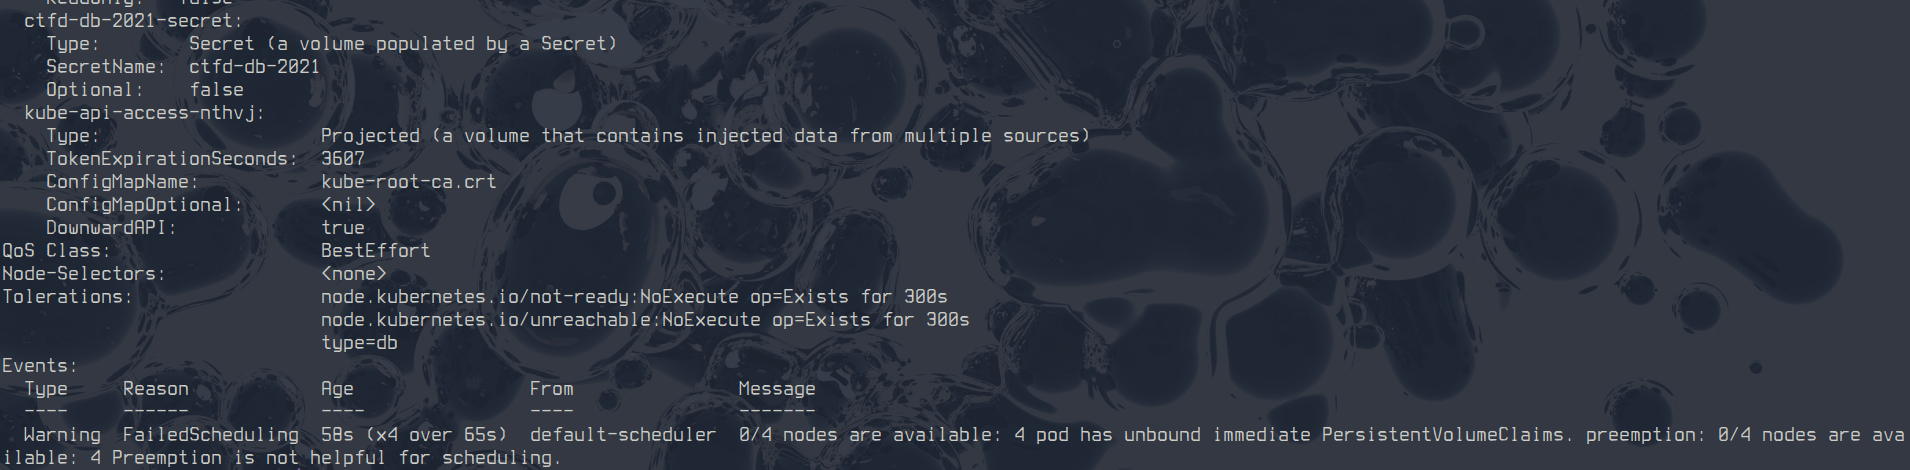
\includegraphics[width=\textwidth]{Kubectl_describe}
	\caption{Motivo de falha do banco de dados}
\end{figure}
\end{frame}

\begin{frame}
\frametitle{Logs}
Possibilita ver a causa de erro dentro do container:
\begin{figure}[htpb]
	\centering
	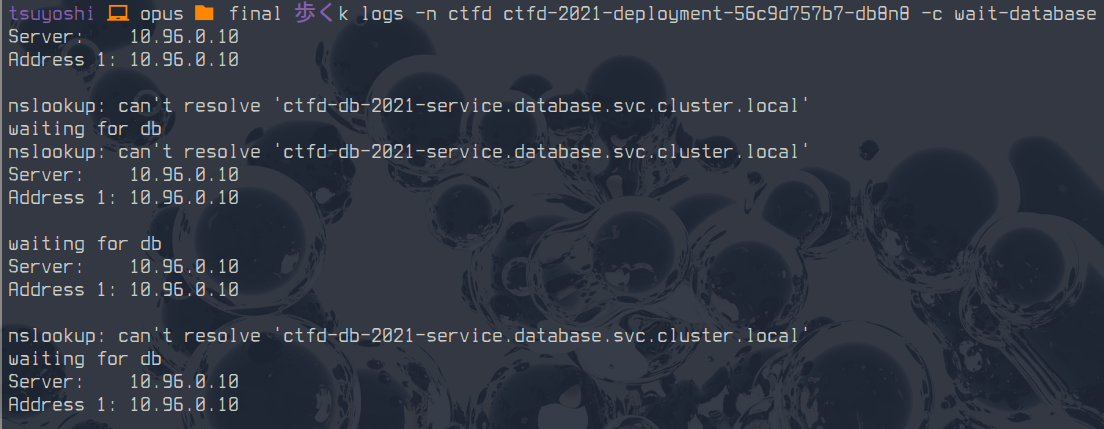
\includegraphics[width=\textwidth]{Kubectl_logs}
	\caption{Log do \textit{initContiner}}
\end{figure}
\end{frame}

\begin{frame}
\frametitle{exec}
Verificar \textit{Mounts, secrets, env, conexão, etc\dots}:
\begin{figure}[htpb]
	\centering
	\includegraphics[width=\textwidth]{Kubernetes_exec}
	\caption{Verificar variáveis de ambiente}
\end{figure}
\end{frame}

\begin{frame}
\frametitle{events}
\begin{itemize}
	\item Os eventos são um relatório de um evento que ocorreu dentro do \textit{cluster}
	\item \uncover<2->{Os eventos são informativos e infomações adicionais}
\end{itemize}

\uncover<3->{
\begin{figure}[htpb]
	\centering
	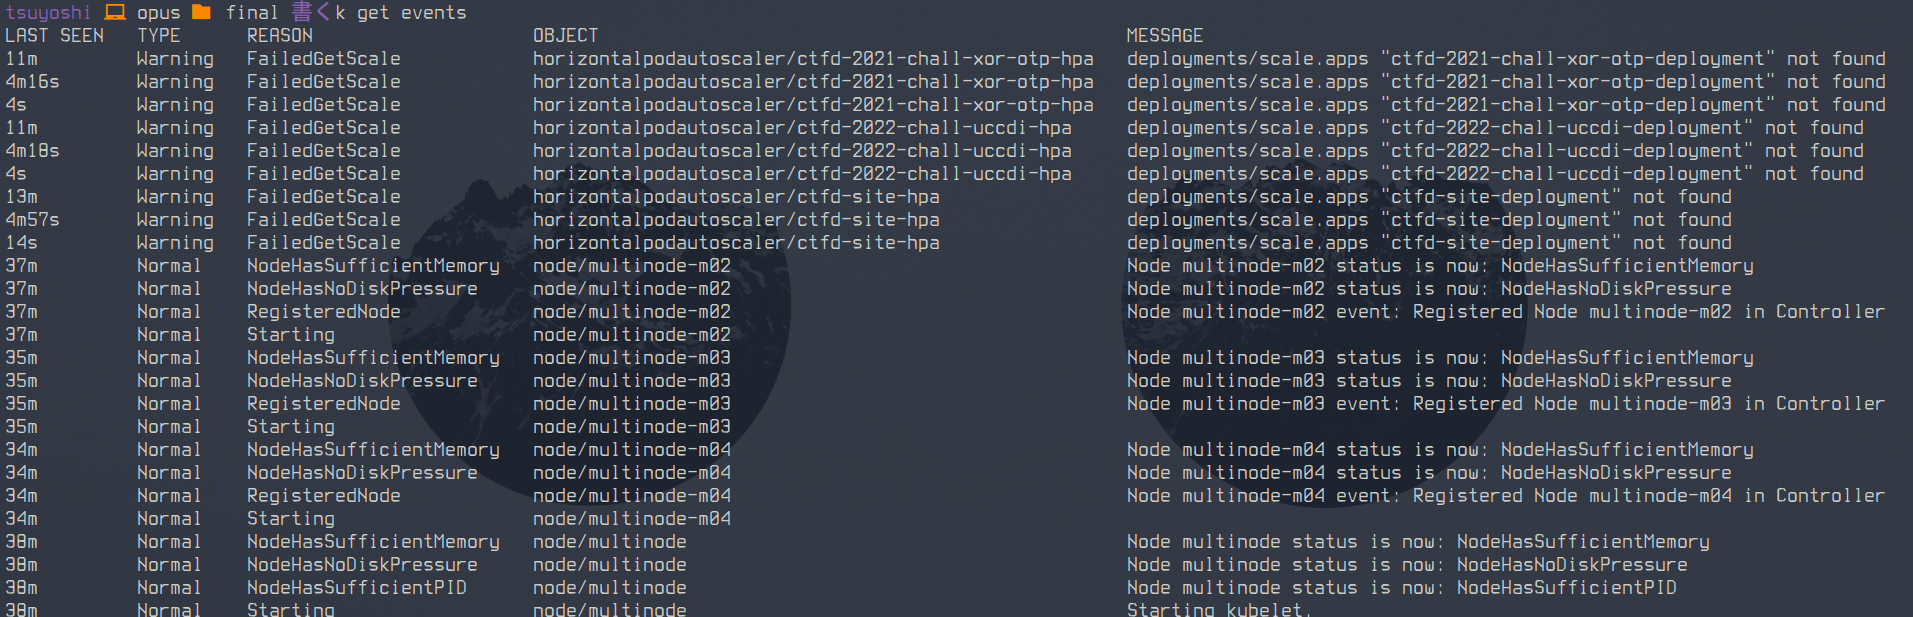
\includegraphics[width=\textwidth]{Kubectl_events}
	\caption{Eventos}
\end{figure}
}
\end{frame}

\section{Ambientes Produtivos}

\begin{frame}
\frametitle{Considerações}
Ambientes produtivos: setup de alta disponibilidade, scaling, quais cuidados tomar, etc
\end{frame}

\begin{frame}
\frametitle{Disponibilidade e Escalabilidade}

Para criar um \textit{cluster} de alta disponibilidade:

\begin{itemize}
	\item Separar \textit{control plane} do nó dos \textit{workers}
	\item Replicar os componentes do \textit{control plane} em multiplos nós
	\item Balancear o tráfico de rede na \textit{API} do \textit{cluster}
	\item Ter nós \textit{workers} suficientes ou ter nós que conseguem ficar disponíveis rapidamente
\end{itemize}

Escalabilidade

\begin{itemize}
	\item Ser capaz de receber as demandas que a aplicação recebe normalmente
	\item Ser capaz de aguentar as demandas em eventos especiais ou datas comemorativas
	\item Planejar como escalar ou reduzir os recursos do \textit{control plane} e dos \textit{workers}
\end{itemize}
\end{frame}

\begin{frame}
\frametitle{Segurança e controle de acesso}
Security and access management: You have full admin privileges on your own Kubernetes learning cluster. But shared clusters with important workloads, and more than one or two users, require a more refined approach to who and what can access cluster resources. You can use role-based access control (RBAC) and other security mechanisms to make sure that users and workloads can get access to the resources they need, while keeping workloads, and the cluster itself, secure. You can set limits on the resources that users and workloads can access by managing policies and container resources.
\end{frame}

Production cluster setup
In a production-quality Kubernetes cluster, the control plane manages the cluster from services that can be spread across multiple computers in different ways. Each worker node, however, represents a single entity that is configured to run Kubernetes pods.

Production control plane
The simplest Kubernetes cluster has the entire control plane and worker node services running on the same machine. You can grow that environment by adding worker nodes, as reflected in the diagram illustrated in Kubernetes Components. If the cluster is meant to be available for a short period of time, or can be discarded if something goes seriously wrong, this might meet your needs.

If you need a more permanent, highly available cluster, however, you should consider ways of extending the control plane. By design, one-machine control plane services running on a single machine are not highly available. If keeping the cluster up and running and ensuring that it can be repaired if something goes wrong is important, consider these steps:

Choose deployment tools: You can deploy a control plane using tools such as kubeadm, kops, and kubespray. See Installing Kubernetes with deployment tools to learn tips for production-quality deployments using each of those deployment methods. Different Container Runtimes are available to use with your deployments.
Manage certificates: Secure communications between control plane services are implemented using certificates. Certificates are automatically generated during deployment or you can generate them using your own certificate authority. See PKI certificates and requirements for details.
Configure load balancer for apiserver: Configure a load balancer to distribute external API requests to the apiserver service instances running on different nodes. See Create an External Load Balancer for details.
Separate and backup etcd service: The etcd services can either run on the same machines as other control plane services or run on separate machines, for extra security and availability. Because etcd stores cluster configuration data, backing up the etcd database should be done regularly to ensure that you can repair that database if needed. See the etcd FAQ for details on configuring and using etcd. See Operating etcd clusters for Kubernetes and Set up a High Availability etcd cluster with kubeadm for details.
Create multiple control plane systems: For high availability, the control plane should not be limited to a single machine. If the control plane services are run by an init service (such as systemd), each service should run on at least three machines. However, running control plane services as pods in Kubernetes ensures that the replicated number of services that you request will always be available. The scheduler should be fault tolerant, but not highly available. Some deployment tools set up Raft consensus algorithm to do leader election of Kubernetes services. If the primary goes away, another service elects itself and take over.
Span multiple zones: If keeping your cluster available at all times is critical, consider creating a cluster that runs across multiple data centers, referred to as zones in cloud environments. Groups of zones are referred to as regions. By spreading a cluster across multiple zones in the same region, it can improve the chances that your cluster will continue to function even if one zone becomes unavailable. See Running in multiple zones for details.
Manage on-going features: If you plan to keep your cluster over time, there are tasks you need to do to maintain its health and security. For example, if you installed with kubeadm, there are instructions to help you with Certificate Management and Upgrading kubeadm clusters. See Administer a Cluster for a longer list of Kubernetes administrative tasks.
To learn about available options when you run control plane services, see kube-apiserver, kube-controller-manager, and kube-scheduler component pages. For highly available control plane examples, see Options for Highly Available topology, Creating Highly Available clusters with kubeadm, and Operating etcd clusters for Kubernetes. See Backing up an etcd cluster for information on making an etcd backup plan.

Production worker nodes
Production-quality workloads need to be resilient and anything they rely on needs to be resilient (such as CoreDNS). Whether you manage your own control plane or have a cloud provider do it for you, you still need to consider how you want to manage your worker nodes (also referred to simply as nodes).

Configure nodes: Nodes can be physical or virtual machines. If you want to create and manage your own nodes, you can install a supported operating system, then add and run the appropriate Node services. Consider:
The demands of your workloads when you set up nodes by having appropriate memory, CPU, and disk speed and storage capacity available.
Whether generic computer systems will do or you have workloads that need GPU processors, Windows nodes, or VM isolation.
Validate nodes: See Valid node setup for information on how to ensure that a node meets the requirements to join a Kubernetes cluster.
Add nodes to the cluster: If you are managing your own cluster you can add nodes by setting up your own machines and either adding them manually or having them register themselves to the cluster’s apiserver. See the Nodes section for information on how to set up Kubernetes to add nodes in these ways.
Scale nodes: Have a plan for expanding the capacity your cluster will eventually need. See Considerations for large clusters to help determine how many nodes you need, based on the number of pods and containers you need to run. If you are managing nodes yourself, this can mean purchasing and installing your own physical equipment.
Autoscale nodes: Most cloud providers support Cluster Autoscaler to replace unhealthy nodes or grow and shrink the number of nodes as demand requires. See the Frequently Asked Questions for how the autoscaler works and Deployment for how it is implemented by different cloud providers. For on-premises, there are some virtualization platforms that can be scripted to spin up new nodes based on demand.
Set up node health checks: For important workloads, you want to make sure that the nodes and pods running on those nodes are healthy. Using the Node Problem Detector daemon, you can ensure your nodes are healthy.
Production user management
In production, you may be moving from a model where you or a small group of people are accessing the cluster to where there may potentially be dozens or hundreds of people. In a learning environment or platform prototype, you might have a single administrative account for everything you do. In production, you will want more accounts with different levels of access to different namespaces.

Taking on a production-quality cluster means deciding how you want to selectively allow access by other users. In particular, you need to select strategies for validating the identities of those who try to access your cluster (authentication) and deciding if they have permissions to do what they are asking (authorization):

Authentication: The apiserver can authenticate users using client certificates, bearer tokens, an authenticating proxy, or HTTP basic auth. You can choose which authentication methods you want to use. Using plugins, the apiserver can leverage your organization’s existing authentication methods, such as LDAP or Kerberos. See Authentication for a description of these different methods of authenticating Kubernetes users.
Authorization: When you set out to authorize your regular users, you will probably choose between RBAC and ABAC authorization. See Authorization Overview to review different modes for authorizing user accounts (as well as service account access to your cluster):
Role-based access control (RBAC): Lets you assign access to your cluster by allowing specific sets of permissions to authenticated users. Permissions can be assigned for a specific namespace (Role) or across the entire cluster (ClusterRole). Then using RoleBindings and ClusterRoleBindings, those permissions can be attached to particular users.
Attribute-based access control (ABAC): Lets you create policies based on resource attributes in the cluster and will allow or deny access based on those attributes. Each line of a policy file identifies versioning properties (apiVersion and kind) and a map of spec properties to match the subject (user or group), resource property, non-resource property (/version or /apis), and readonly. See Examples for details.
As someone setting up authentication and authorization on your production Kubernetes cluster, here are some things to consider:

Set the authorization mode: When the Kubernetes API server (kube-apiserver) starts, the supported authentication modes must be set using the --authorization-mode flag. For example, that flag in the kube-adminserver.yaml file (in /etc/kubernetes/manifests) could be set to Node,RBAC. This would allow Node and RBAC authorization for authenticated requests.
Create user certificates and role bindings (RBAC): If you are using RBAC authorization, users can create a CertificateSigningRequest (CSR) that can be signed by the cluster CA. Then you can bind Roles and ClusterRoles to each user. See Certificate Signing Requests for details.
Create policies that combine attributes (ABAC): If you are using ABAC authorization, you can assign combinations of attributes to form policies to authorize selected users or groups to access particular resources (such as a pod), namespace, or apiGroup. For more information, see Examples.
Consider Admission Controllers: Additional forms of authorization for requests that can come in through the API server include Webhook Token Authentication. Webhooks and other special authorization types need to be enabled by adding Admission Controllers to the API server.
Set limits on workload resources
Demands from production workloads can cause pressure both inside and outside of the Kubernetes control plane. Consider these items when setting up for the needs of your cluster's workloads:

Set namespace limits: Set per-namespace quotas on things like memory and CPU. See Manage Memory, CPU, and API Resources for details. You can also set Hierarchical Namespaces for inheriting limits.
Prepare for DNS demand: If you expect workloads to massively scale up, your DNS service must be ready to scale up as well. See Autoscale the DNS service in a Cluster.
Create additional service accounts: User accounts determine what users can do on a cluster, while a service account defines pod access within a particular namespace. By default, a pod takes on the default service account from its namespace. See Managing Service Accounts for information on creating a new service account. For example, you might want to:
Add secrets that a pod could use to pull images from a particular container registry. See Configure Service Accounts for Pods for an example.
Assign RBAC permissions to a service account. See ServiceAccount permissions for details.
What's next
Decide if you want to build your own production Kubernetes or obtain one from available Turnkey Cloud Solutions or Kubernetes Partners.
If you choose to build your own cluster, plan how you want to handle certificates and set up high availability for features such as etcd and the API server.
Choose from kubeadm, kops or Kubespray deployment methods.
Configure user management by determining your Authentication and Authorization methods.
Prepare for application workloads by setting up resource limits, DNS autoscaling and service accounts.


\section{Helm}

\begin{frame}
\frametitle{Helm}
\begin{center}
\textbf{"Helm helps you manage Kubernetes applications — Helm Charts help you define, install, and upgrade even the most complex Kubernetes application."} \cite{Helm}
\begin{itemize}
	\uncover<2->{\item Instalar charts}
	\uncover<3->{\item Criar charts}
	\uncover<4->{\item Remover charts}
	\uncover<5->{\item Escolher repositórios}
\end{itemize}
\end{center}
\end{frame}

\begin{frame}
\frametitle{Charts}
\begin{center}
\textbf{"Charts are easy to create, version, share, and publish — so start using Helm and stop the copy-and-paste."} \cite{Helm}
\begin{itemize}
	\uncover<2->{\item Criar}
	\uncover<3->{\item Versionar}
	\uncover<4->{\item Compartilhar}
	\uncover<5->{\item Publicar}
\end{itemize}
\end{center}
\end{frame}

\begin{frame}[containsverbatim]
\frametitle{Helm}
\begin{center}
\begin{minipage}{0.9\textwidth}
\begin{block}{Instalar o \textit{Redis}}
\begin{lstlisting}[language=bash]
helm install ctfd-redis -f ./redis/values.yaml \
-n redis \
bitnami/redis
\end{lstlisting}
\end{block}
\end{minipage}
\end{center}
Instalar o \textit{redis} no namespace \textbf{redis} com os valores \textbf{./redis/values.yaml} do repositório \textbf{\url{https://charts.bitnami.com/bitnami}}
\end{frame}

\begin{frame}[containsverbatim]
\frametitle{Helm}
Como foi utilizado no projeto:
\begin{center}
\begin{minipage}{0.9\textwidth}
\begin{block}{\textbf{values.yaml}}
\begin{lstlisting}
architecture: standalone
auth:
  enabled: false
master:
  tolerations:
    - key: "type"
      operator: "Equal"
      value: "db"
  securityContext:
    enabled: true
    fsGroup: 2000
    runAsUser: 0
\end{lstlisting}
\end{block}
\end{minipage}
\end{center}
\end{frame}

\begin{frame}[containsverbatim]
\frametitle{Helm}
\begin{center}
\begin{minipage}{0.9\textwidth}
\begin{block}{\textbf{values.yaml}}
\begin{lstlisting}
master:
  persistence:
    enabled: true
    storageClass: "nfs"
    accessModes:
    - ReadWriteOnce
    size: 8Gi
    matchLabels:
      name: ctfd-redis-pv
\end{lstlisting}
\end{block}
\end{minipage}
\end{center}
\end{frame}

\section{Referencias}

\begin{frame}
\frametitle{Referencias}
\printbibliography
\end{frame}




\end{document}
